% Copyright (c) 2014,2016 Casper Ti. Vector
% Public domain.

\chapter{基于区块链的命名实体鉴权系统实现}

本章将给出本文提出方案的一种实现方法,首先对方案实现的系统设计进行阐述,叙述实现本方案的方法以及本文选择实现方法的原理;其后给出系统实现的模块模块设计...

\section{系统设计}

本章将对方案实现的这个系统进行描述,涉及到系统中的各个角色要求和功能;然后给出系统实现的整体架构,从上层透视系统中的信息交互;最后给出实现本系统的方式建议和本文所采用的方法及其原因。

\subsection{系统角色}


在方案设计的章节中,我们通过对现有PKI系统中相关实体的描述,结合方案设计的目标和相关的操作,可以得知,在实现过程中涉及的实体主要包括以下四类:作为证书申请者的用户(即域名)、依赖方、参与到系统中的验证节点、以及区块链的全节点。

根据方案设计中的内容,不同实体加入到本系统中拥有各自的目的;并且对于不同实体,其对本系统起到的作用和能够完成的操作也各不相同,下面将对它们加入本系统的目的和存在的意义进行介绍。

\noindent\textbf{用户}

域名作为本方案的用户,其希望通过本系统完成对自己可信CA的控制,达到防止未经允许的恶意CA对其签发证书的目的。

在本系统中,所有的数据都是通过区块链来存储的,域名和所有参与者一样在区块链上的身份都是不具有代表性。为了建立域名在区块链上的身份(公钥或者地址)和自身的联系,需要通过上一章中设计的身份鉴权方案进行身份的绑定;在其完成使用公钥和自身身份的绑定后,就可以通过区块链上的身份来完成对域名标识的信任CA控制,在区块链对可信CA列表进行管理操作。综上,在域名在本系统需要完成两个操作,其一是在区块链上完成身份绑定操作;其二是完成可信CA列表的管理操作。


\noindent\textbf{依赖方}

依赖方通过游览器在PKI系统完成的通信工作,需要对证书的有效性进行检查。在本方案中,需要通过区块链进一步确认证书是否被合理的签发,为依赖方提供证书的进一步检查,达到其不被恶意签发证书所欺骗的作用。

在本系统中,依赖方所需要完成的操作相对比较简单,只需要本系统中的区块链网络中获取通信实体的可信CA列表即可,然后与收到的证书签发方进行对比,验证其是否存在与可信CA列表之中,如果不存在则需要向依赖方发出警告提示。


\noindent\textbf{验证节点}

验证节点加入到本系统中的目的是为了获取验证过程中产生的奖励。

验证节点在本系统起着至关重要的作用,是否有住够多的验证节点加入到本系统中,决定着本系统是否能够有效的运行下去。在本系统中,验证节点需要对域名发起的身份验证请求进行验证,帮助它们完成区块链上身份与域名真实身份的绑定操作。根据方案设计可知,验证节点为了自身利益,需要实时的监控区块链上发起的验证交易,判断自己是否能够成为验证节点并获得相应的奖励,所以验证节点在本方案中需要完成操作包括监控区块链上的交易和对交易的验证。

\noindent\textbf{全节点}

全节点加入到本系统的目的是为了完成对区块链的维护,从而获得相应的奖励。

全节点作为区块链系统中的完整节点,实时的监控整个网络中的所有交易,并尝试这些交易打包到最新的区块链中去。每当完成一个区块的创建,将会获得区块链挖矿所分配的奖励。对于本系统而言,它们是底层区块链平台的维护者,为上面的所有实体提供了基础平台。


在系统中的单个实体可以扮演以上的单个或者多个角色,比如域名作为本系统中的用户,可以成为本系统中的验证节点或者全节点,为本系统正常运行做出贡献的同事,也可以从中获得相应的奖励。普通的网页游览用户,通过游览器进行网页游览并发起对域名证书的二次验证,确保自身的权益,同时也可以成为本系统中的验证节点和全节点。



\subsection{系统架构}

在上一小节中,我们对系统中涉及的角色进行了描述,在本小节中我们将给出系统的整体结构,给出系统中的相关组件,并阐述角色和组件之间如何协作。

本系统中涉及的角色包括域名、依赖方、验证节点以及全节点,通过区块链网络连接到一起,共同参与到本系统之中,系统的整体架构如图\ref{fig:framework}所示。




\begin{figure}[htbp]
 	\centering
 	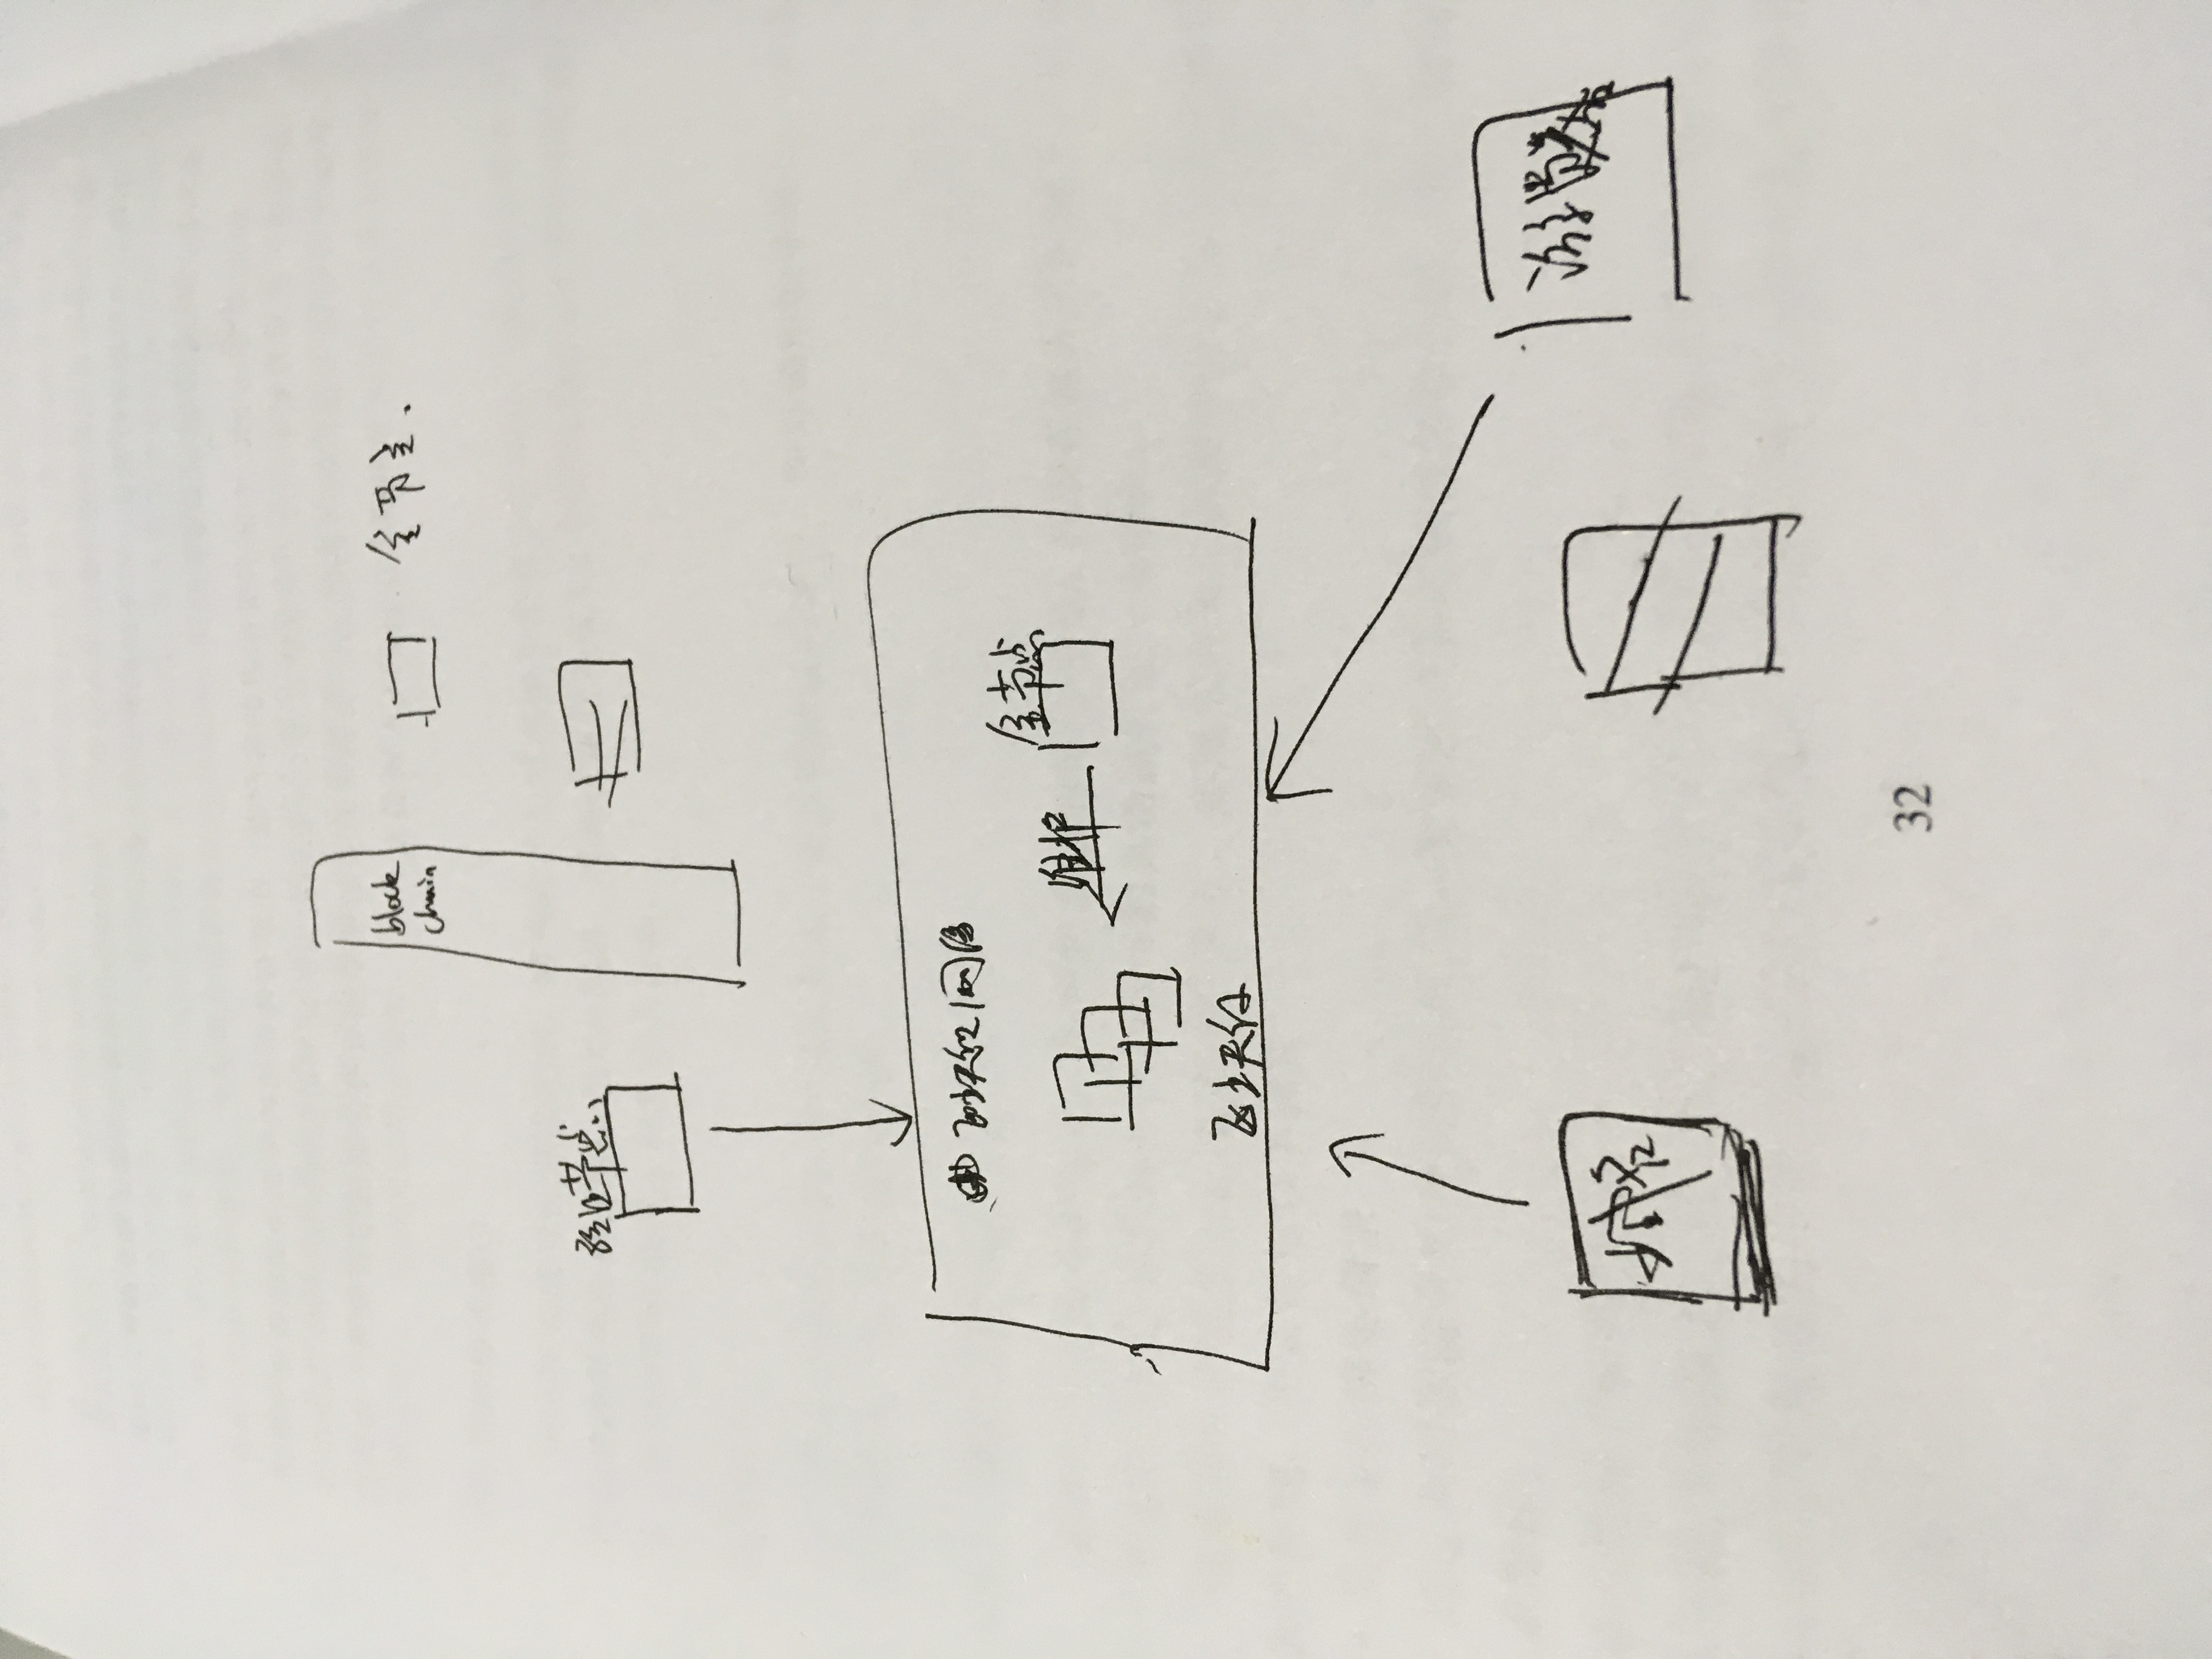
\includegraphics[width = 0.8\textwidth]{img/system_framework}
 	\caption{系统架构}\label{fig:framework}
\end{figure}



在本系统中,区块全是整个系统的重心,所有参与大本系统中的角色都要通过其进行关联。不同的角色之间需要使用不同的工具来完成与区块链网络的交互,依赖方在传统PKI系统中使用的是游览器来完成对证书的检验,同样,在本系统也依赖与游览器中的插件来完成对证书的二次验证;对于域名而言,需要有相应的客户端来与区块链进行交互,完成验证请求的发布和相关验证信息的部署;验证节点同样需要有相应的客户端来获取区块链上所提交的验证请求,并通过客户端来判断自己是否能够完成验证请求,对验证请求进行响应;作为维护区块链的全节点,则直接通过区块链的客户端进行区块链维护工作即可。

\subsection{实现方式}

本文所提及的方案中是依托于区块链及其上面的用户实体的,所以必须需要一个区块链平台才能完成上述系统的构建,以实现本文提出的方案。在我看来,实现以上系统有两种方式:一种是利用已有的区块链平台,通过其上的智能合约来完成本文给出方案的相关逻辑和操作;另外一种方式是重新构建一个全新的区块链平台,依据本文中给出方案去设计区块链平台的功能和相关交易,已完成上述实体之间的信息交互。

以上提到的两种方式都可以完成本系统的构建,且只是影响该系统中的底层区块链的构建,对上层如域名、依赖方以及验证节点并没有实质性的影响,仅仅是通过不同的方式去访问不同的区块链网络给。但是两种不同的实现方式各有利弊额,如表\ref{cmpMethod}所示。

\begin{table}[h] \label{cmpMethod}%开始一个表格environment,表格的位置是h,here。  
\caption{实现方式对比} %显示表格的标题  
\begin{tabular}{l*{6}{c}} %设置了每一列的宽度,强制转换。  
\hline  
\hline  
  & 难度 & 工程量 & 网络建立速度 & 性能 & 独立性 & 全节点维护代价 \\ %用&来分隔单元格的内容 \\表示进入下一行  
\hline %画一个横线,下面的就都是一样了,这里一共有4行内容  
基于智能合约 & 低 & 小 & 快 & 低 & 低 & 高 \\
\hline  
创建新链 & 高 & 大 & 慢 & 高 & 高 & 小 \\
 
\hline  
\hline  
\end{tabular}  
\end{table}  

基于智能合约的方式相比于创建新链的方式而言,实现起来可能更加容易,不需要对区块链的底层去进行修改,只需要在上次的智能合约中完成相关功能和模块即可,所以难度更小;同时,基于智能合约的方式需要书写的代码也要少一些,因而具有工程量更小。由于基于享有的区块链平台去开发智能合约,该平台一般情况下已经积累了一定的用户,很多节点已经在上面进行区块链的维护;而新开发一条链需要一段时间才能有住够多的用户加入到其中,保证该系统能够安全有效的进行下去;因此,系统建立的速度而言,基于智能合约方式更加高效。

但是,基于智能合约的方式也存在着相应的缺点,主要是性能、健壮性和全节点付出的代价。由于现有的支持智能合约的公链的性能都很低,并且其上还充斥这其它智能合约的交易,所以在其上开发智能合约会直接导致本系统的请求处理并不会那么快,性能会比较低下;而创建一条新链,这可以通过一系列优化来提高其性能;另外一个问题就是整个系统的独立性并不好,很大程度上要取决于依赖的区块链平台,如果该平台出现一些问题,那么将直接影响到本系统的正常工作;最后是全节点付出的代价问题,如果一个全节点想维护本系统中的账本,那么其必须要将该区块链上的所有交易记录都维护下来,包含了一下其它不是很相关的交易,大大提高了其加入本系统的代价。

本文将选择基于智能合约的方式实现,在以太坊上通过智能合约完成相关功能的实现。



\section{模块设计}


本方案以区块链作为底层架构,在其上需要上述方案中的相关逻辑,让PKI中的相关实体与区块链进行交互,在其上完成身份认证并进行相关数据的存储,实现对域名可信CA列表的访问与控制,并最终完成证书有效性的进一步确认。

根据上面的设计,本系统如\ref{fig:module}图分为四个模块进行实现:智能合约、域名客户端、验证节点客户端、游览器验证插件。

\begin{figure}[htbp]
 	\centering
 	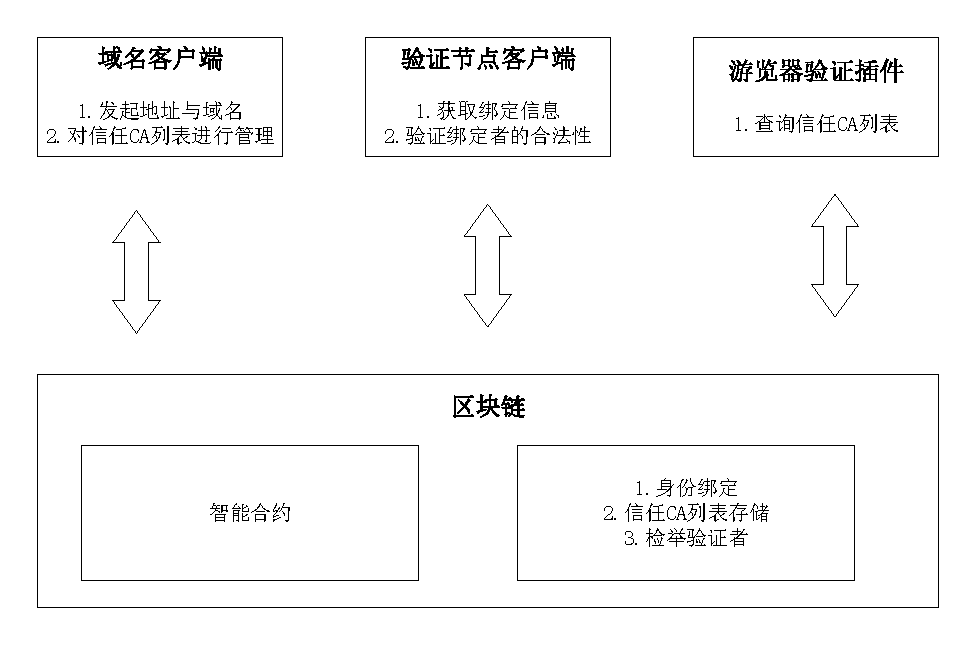
\includegraphics[width = 0.8\textwidth]{img/module}
 	\caption{系统模块设计}\label{fig:module}
\end{figure}

\subsection{智能合约}

智能合约作为可以在区块链上实现其他逻辑操作的一种工具,在本部分,将给予以太坊作为底层区块链基础,在其上开发具有本文所述方案的智能合约,提供其它模块访问区块链的相关接口和功能,完成本文所述方案中的逻辑操作。

区块链作为本方案的信息流转媒介,其上不仅要完成对域名信任CA的相关信息存储,还需要完成域名认证的操作。根据区块链要实现的功能,该模块需要提供身份绑定接口、信任列表修改接口、信任列表存储接口以及检举接口。

\subsubsection{身份绑定接口}

身份绑定接口主要提供给域名客户端和验证节点客户端使用,针对不同的客户端有两种不同的的操作:身份绑定请求和身份绑定确认。

身份绑定请求操作是由域名通过域名客户端发起,发送需要绑定的域名和公钥到智能合约中进行登记,并放置合法的验证内容到自己的服务器上,供验证节点对其进行验证。

在身份绑定请求发送成功之后,验证节点客户端可以获得最新的待验证身份绑定信息,并对身份绑定的信息进行验证,如果验证通过,则会通过智能合约调用身份绑定确认操作,完成身份绑定验证。

\subsubsection{信任列表修改接口}

域名在完成身份绑定之后,即拥有了与域名相关联的公私钥对,通过对公钥对应内容的控制调整自己信任的CA列表。其通过调用信任CA列表对信任CA进行修改操作,并存储在区块链上供其它人查阅。


\subsubsection{检举接口}

当验证者发现带确认的域名并未正确放置验证内容时,即可调用检举接口,完成对公钥对本次域名绑定的检举。

\subsection{域名客户端}

域名作为证书的申请者,需要将自己的可信任CA列表存储到区块链上,以供证书受用者在使用证书的过程中对证书的真伪进行进一步检查。

域名客户端需要与区块链进行交互,实现域名和公钥的绑定以及对自己可信CA列表的控制,主要包括以下操作:

\begin{itemize}
	\item 

	发起身份绑定请求

	通过调用身份绑定接口,发送需要绑定的域名和公钥,完成身份绑定请求操作。

	\item 

	修改信任CA列表

	在完成身份绑定之后,域名客户端将可以控制公钥和域名所对应的信任CA列表,通过调用信任列表修改接口,完成对自身信任CA列表的管控。


\end{itemize}

\subsection{验证节点客户端}

验证节点是本系统中身份鉴权的重要组成部分,是身份绑定有效性的保证,只有住够多验证节点存在的情况下,才可以保证身份确认的有效。

验证节点的主要工作是实时的查询验证请求并对验证请求进行验证,并根据其验证请求计算自己是否符合验证节点的要求,如果符合的话将进行验证确认操作,如果不是,也可以进行验证,对不符的验证提交检举交易。


\subsection{游览器验证插件}


游览器是Web PKI中证书受用者的客户端,在原有体系结构中充当着检查证书真伪的角色。在本方案中,为了保证被恶意CA私自签发的证书可以被识别出来,需要在客户端进行对证书进行额外的检查,也就是需要游览器需要有区块链进行交互,查询收到的证书是否由证书申请者信任的CA所签发。

% vim:ts=4:sw=4
